
%(BEGIN_QUESTION)
% Copyright 2006, Tony R. Kuphaldt, released under the Creative Commons Attribution License (v 1.0)
% This means you may do almost anything with this work of mine, so long as you give me proper credit

An ingenious circuit used to convert the output of a differential capacitance sensor into a DC voltage signal is the {\it diode twin-t circuit} shown here:

$$\includegraphics[width=15.5cm]{i00186x01.eps}$$

The AC ``excitation'' voltage source is typically of high frequency, at least 1 MHz.  The diodes are fast-switching units, ideally Schottky diodes.  Resistors $R$ must be equal in value, but $R_{load}$ is usually much greater than $R$.  Together, the two matched resistors ($R$) form an {\it averaging network} for the two capacitances $C$ and $C'$ as they alternately discharge through $R_{load}$.

Identify which capacitance ($C$ or $C'$) must increase in value to generate a positive DC output voltage, and why this is so.

\underbar{file i00186}
%(END_QUESTION)





%(BEGIN_ANSWER)

The output voltage will be positive with respect to ground if $C > C'$ and negative if $C' > C$.

%(END_ANSWER)





%(BEGIN_NOTES)

I cannot take credit for this wonderful little circuit.  I found it on page 72 of {\it Principles of Applied Biomedical Instrumentation} by Geddes and Baker (Copyright 1968, John Wiley and Sons).  Having used it in my own differential-capacitance manometer, I can assure you it works very well:

$$\includegraphics[width=15.5cm]{i00186x02.eps}$$

This is a relatively easy instrument to make out of rigid copper tubing.  Use plastic compression-style tube fittings for the insulating bushings.

\vskip 10pt

It might be good to review this formula with your students in discussing the operation of this capacitance-based instrument:

$$C = {\epsilon A \over d}$$

\noindent
Where,

$C =$ Capacitance in Farads

$\epsilon =$ Permittivity of dielectric (absolute)

$A =$ Conductor area, in square meters

$d =$ Separation distance, in meters


%INDEX% Measurement, differential capacitance: twin tee diode circuit

%(END_NOTES)


